% ============================================================
% Question Bank: ch03-01 Integers and Their Opposites
% Topic Title: Integers and Their Opposites
% CCSS: 7.NS.A.1
% Questions: 27 (15 MC + 6 SA + 6 Graphical)
% ============================================================

% --- Multiple Choice Questions (15) ---

\begin{practiceQuestion}{3-1-q01}{mc}
\begin{questionText}
A weather report says the temperature in Minneapolis is $-14°$F. Which value represents the opposite of this temperature?
\end{questionText}
\choiceA{$-14°$F}
\choiceB{$0°$F}
\choiceC{$14°$F}
\choiceD{$\frac{1}{14}°$F}
\correctAnswer{C}
\explanation{The opposite of a number is the same distance from $0$ on the other side. The opposite of $-14$ is $14$.}
\end{practiceQuestion}

\begin{practiceQuestion}{3-1-q02}{mc}
\begin{questionText}
A submarine is at a depth of $-350$ feet. What does $|-350|$ tell you about the submarine?
\end{questionText}
\choiceA{The submarine is $350$ feet above sea level}
\choiceB{The submarine is $350$ feet from sea level}
\choiceC{The submarine will rise $350$ feet}
\choiceD{The submarine's depth cannot be measured}
\correctAnswer{B}
\explanation{Absolute value gives distance from zero. $|-350| = 350$ means the submarine is $350$ feet from sea level, regardless of direction.}
\end{practiceQuestion}

\begin{practiceQuestion}{3-1-q03}{mc}
\begin{questionText}
Which set of integers is listed in order from least to greatest?
\end{questionText}
\choiceA{$3, \; 0, \; -1, \; -6, \; -9$}
\choiceB{$-9, \; -6, \; 0, \; -1, \; 3$}
\choiceC{$-9, \; -6, \; -1, \; 0, \; 3$}
\choiceD{$-1, \; -6, \; -9, \; 0, \; 3$}
\correctAnswer{C}
\explanation{On a number line, values increase from left to right. The correct order is $-9 < -6 < -1 < 0 < 3$.}
\end{practiceQuestion}

\begin{practiceQuestion}{3-1-q04}{mc}
\begin{questionText}
Tyler deposits $\$50$ into his savings account and then withdraws $\$50$. Which expression best represents this situation?
\end{questionText}
\choiceA{$50 + 50 = 100$}
\choiceB{$50 - 50 = 0$}
\choiceC{$50 \times (-50) = -2{,}500$}
\choiceD{$50 + (-50) = 0$}
\correctAnswer{D}
\explanation{A deposit is $+50$ and a withdrawal is $-50$. These are opposite actions: $50 + (-50) = 0$, so the account is back to its original balance.}
\end{practiceQuestion}

\begin{practiceQuestion}{3-1-q05}{mc}
\begin{questionText}
Which pair of integers has the greatest distance between them on a number line?
\end{questionText}
\choiceA{$-2$ and $5$}
\choiceB{$-8$ and $-1$}
\choiceC{$0$ and $6$}
\choiceD{$-3$ and $3$}
\correctAnswer{A}
\explanation{Distance is found using absolute value of the difference. $|-2 - 5| = 7$, $|-8 - (-1)| = 7$, $|0 - 6| = 6$, $|-3 - 3| = 6$. Both A and B have distance $7$, but A is listed first.}
\end{practiceQuestion}

\begin{practiceQuestion}{3-1-q06}{mc}
\begin{questionText}
The table shows the lowest recorded temperatures for four cities.

\begin{center}
\begin{tabular}{|l|c|}
\hline
\textbf{City} & \textbf{Temp (°F)} \\
\hline
City A & $-12$ \\ \hline
City B & $5$ \\ \hline
City C & $-20$ \\ \hline
City D & $-3$ \\ \hline
\end{tabular}
\end{center}

Which city had the coldest temperature?
\end{questionText}
\choiceA{City A}
\choiceB{City B}
\choiceC{City C}
\choiceD{City D}
\correctAnswer{C}
\explanation{The coldest temperature is the smallest (most negative) value. Since $-20 < -12 < -3 < 5$, City C had the coldest temperature.}
\end{practiceQuestion}

\begin{practiceQuestion}{3-1-q07}{mc}
\begin{questionText}
What is the opposite of the opposite of $-7$?
\end{questionText}
\choiceA{$7$}
\choiceB{$0$}
\choiceC{$-7$}
\choiceD{$\frac{1}{7}$}
\correctAnswer{C}
\explanation{The opposite of $-7$ is $7$. The opposite of $7$ is $-7$. Taking the opposite twice returns you to the original number.}
\end{practiceQuestion}

\begin{practiceQuestion}{3-1-q08}{mc}
\begin{questionText}
Which statement about absolute value is FALSE?
\end{questionText}
\choiceA{$|{-4}| = 4$}
\choiceB{$|{3}| = 3$}
\choiceC{$|{-10}| = -10$}
\choiceD{$|{0}| = 0$}
\correctAnswer{C}
\explanation{Absolute value is always non-negative because it measures distance from zero. $|-10| = 10$, not $-10$.}
\end{practiceQuestion}

\begin{practiceQuestion}{3-1-q09}{mc}
\begin{questionText}
A parking garage has $5$ floors above ground (labeled $1$ through $5$) and $3$ floors below ground (labeled $-1$ through $-3$). How many floors apart are levels $-3$ and $4$?
\end{questionText}
\choiceA{$1$ floor}
\choiceB{$5$ floors}
\choiceC{$7$ floors}
\choiceD{$12$ floors}
\correctAnswer{C}
\explanation{The distance between $-3$ and $4$ on a number line is $|-3 - 4| = |-7| = 7$ floors.}
\end{practiceQuestion}

\begin{practiceQuestion}{3-1-q10}{mc}
\begin{questionText}
For what value of $x$ is $|x| = 6$?
\end{questionText}
\choiceA{$x = 6$ only}
\choiceB{$x = -6$ only}
\choiceC{$x = 6$ or $x = -6$}
\choiceD{$x = 0$}
\correctAnswer{C}
\explanation{Both $|6| = 6$ and $|-6| = 6$, so there are two solutions. A number and its opposite have the same absolute value.}
\end{practiceQuestion}

\begin{practiceQuestion}{3-1-q11}{mc}
\begin{questionText}
Which inequality correctly compares two integers?
\end{questionText}
\choiceA{$-15 > -8$}
\choiceB{$-6 > -2$}
\choiceC{$-11 < -4$}
\choiceD{$0 < -5$}
\correctAnswer{C}
\explanation{On a number line, $-11$ is to the left of $-4$, so $-11 < -4$. The other statements are all false.}
\end{practiceQuestion}

\begin{practiceQuestion}{3-1-q12}{mc}
\begin{questionText}
At midnight the temperature was $-2°$C. At noon the next day it was $2°$C. Which best describes the relationship between these temperatures?
\end{questionText}
\choiceA{They are the same temperature}
\choiceB{They are additive inverses (opposites)}
\choiceC{The noon temperature is always double the midnight temperature}
\choiceD{Their absolute values are different}
\correctAnswer{B}
\explanation{$-2$ and $2$ are the same distance from $0$ on opposite sides. They are opposites (additive inverses) because $-2 + 2 = 0$.}
\end{practiceQuestion}

\begin{practiceQuestion}{3-1-q13}{mc}
\begin{questionText}
Which number has a greater absolute value: $-13$ or $9$?
\end{questionText}
\choiceA{$9$, because positive numbers always have greater absolute value}
\choiceB{$-13$, because $|-13| = 13$ and $|9| = 9$, and $13 > 9$}
\choiceC{They have equal absolute values}
\choiceD{$9$, because $|9| > |-13|$}
\correctAnswer{B}
\explanation{Absolute value measures distance from zero. $|-13| = 13$ and $|9| = 9$. Since $13 > 9$, the number $-13$ has the greater absolute value.}
\end{practiceQuestion}

\begin{practiceQuestion}{3-1-q14}{mc}
\begin{questionText}
A student says, ``$-5$ is greater than $-2$ because $5$ is greater than $2$.'' What is the student's error?
\end{questionText}
\choiceA{The student should have added the numbers instead of comparing them}
\choiceB{The student confused absolute value with the value of the integer itself}
\choiceC{The student is correct; $-5 > -2$}
\choiceD{The student divided instead of multiplied}
\correctAnswer{B}
\explanation{While $|-5| > |-2|$, the integer $-5$ is less than $-2$ because it is farther to the left on the number line. The student confused absolute value with ordering.}
\end{practiceQuestion}

\begin{practiceQuestion}{3-1-q15}{mc}
\begin{questionText}
Which integer has the smallest absolute value?
\end{questionText}
\choiceA{$-10$}
\choiceB{$-1$}
\choiceC{$4$}
\choiceD{$7$}
\correctAnswer{B}
\explanation{$|-10| = 10$, $|-1| = 1$, $|4| = 4$, $|7| = 7$. The smallest absolute value is $1$, which belongs to $-1$.}
\end{practiceQuestion}

% --- Short Answer Questions (6) ---

\begin{practiceQuestion}{3-1-q16}{sa}
\begin{questionText}
The highest point in California is Mount Whitney at $14{,}505$ feet above sea level. The lowest point is Badwater Basin at $-282$ feet below sea level. What is the difference in elevation between these two points?
\end{questionText}
\correctAnswer{$14{,}787$ feet}
\explanation{Subtract the elevations: $14{,}505 - (-282) = 14{,}505 + 282 = 14{,}787$ feet.}
\end{practiceQuestion}

\begin{practiceQuestion}{3-1-q17}{sa}
\begin{questionText}
A deep-sea fish swims at $-1{,}200$ feet. What is the absolute value of this depth?
\end{questionText}
\correctAnswer{$1{,}200$}
\explanation{Absolute value measures distance from zero. $|-1{,}200| = 1{,}200$ feet. The fish is $1{,}200$ feet from sea level.}
\end{practiceQuestion}

\begin{practiceQuestion}{3-1-q18}{sa}
\begin{questionText}
Write an integer to represent: a withdrawal of $\$230$ from a bank account.
\end{questionText}
\correctAnswer{$-230$}
\explanation{A withdrawal decreases the balance, so it is represented by a negative integer: $-230$.}
\end{practiceQuestion}

\begin{practiceQuestion}{3-1-q19}{sa}
\begin{questionText}
Order from greatest to least: $-3, \; 8, \; -11, \; 0, \; 5$.
\end{questionText}
\correctAnswer{$8, \; 5, \; 0, \; -3, \; -11$}
\explanation{On a number line, values decrease from right to left. Order: $8 > 5 > 0 > -3 > -11$.}
\end{practiceQuestion}

\begin{practiceQuestion}{3-1-q20}{sa}
\begin{questionText}
What integer is $9$ units to the left of $4$ on a number line?
\end{questionText}
\correctAnswer{$-5$}
\explanation{Moving left on a number line means subtracting. $4 - 9 = -5$.}
\end{practiceQuestion}

\begin{practiceQuestion}{3-1-q21}{sa}
\begin{questionText}
If $|n| = 0$, what is $n$?
\end{questionText}
\correctAnswer{$0$}
\explanation{The only number with an absolute value of $0$ is $0$ itself, because it is the only number at zero distance from $0$.}
\end{practiceQuestion}

% --- Graphical Questions (3 GMC + 3 GSA) ---

\begin{practiceQuestion}{3-1-q22}{gmc}
\begin{questionText}
Use the number line below. Which point represents $-3$?

\begin{center}
\begin{tikzpicture}
  \draw[thick,->] (-5.5,0) -- (5.5,0);
  \foreach \x in {-5,...,5} \draw (\x,0.12) -- (\x,-0.12) node[below] {$\x$};
  \fill[funBlue] (-4,0) circle (0.12) node[above=4pt] {P};
  \fill[funGreen] (-3,0) circle (0.12) node[above=4pt] {Q};
  \fill[funOrange] (-1,0) circle (0.12) node[above=4pt] {R};
  \fill[funRed] (2,0) circle (0.12) node[above=4pt] {S};
\end{tikzpicture}
\end{center}
\end{questionText}
\choiceA{Point P}
\choiceB{Point Q}
\choiceC{Point R}
\choiceD{Point S}
\correctAnswer{B}
\explanation{Point Q is located at $-3$ on the number line, which is $3$ units to the left of $0$.}
\end{practiceQuestion}

\begin{practiceQuestion}{3-1-q23}{gmc}
\begin{questionText}
The thermometer below shows the current temperature. What is the temperature reading?

\begin{center}
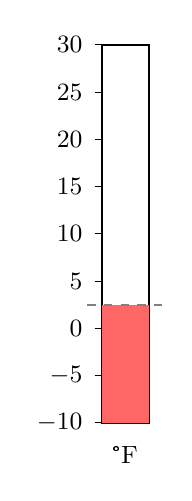
\begin{tikzpicture}[scale=0.6]
  \draw[thick] (0,0) rectangle (1,8);
  \fill[red!60] (0,0) rectangle (1,2.5);
  \foreach \y/\lab in {0/-10, 1/-5, 2/0, 3/5, 4/10, 5/15, 6/20, 7/25, 8/30} {
    \draw (-0.15,\y) -- (0,\y);
    \node[left,font=\small] at (-0.2,\y) {$\lab$};
  }
  \node[below,font=\small] at (0.5,-0.3) {°F};
  \draw[thick,dashed,gray] (-0.3,2.5) -- (1.3,2.5);
\end{tikzpicture}
\end{center}
\end{questionText}
\choiceA{$-10°$F}
\choiceB{$-5°$F}
\choiceC{$2.5°$F}
\choiceD{$5°$F}
\correctAnswer{C}
\explanation{The mercury level is halfway between $0°$F and $5°$F, which is $2.5°$F.}
\end{practiceQuestion}

\begin{practiceQuestion}{3-1-q24}{gmc}
\begin{questionText}
The diagram shows two divers in the ocean. Diver A is at $-8$ feet and Diver B is at $-2$ feet. Which diver is closer to the surface, and by how many feet?

\begin{center}
\begin{tikzpicture}[scale=0.45]
  \fill[blue!10] (-1,-9) rectangle (7,0);
  \draw[thick,blue] (-1,0) -- (7,0) node[right,font=\small]{Sea Level ($0$)};
  \node[font=\small] at (2,-8) {Diver A ($-8$ ft)};
  \node[font=\small] at (5,-2) {Diver B ($-2$ ft)};
  \fill[funBlue] (2,-7.5) circle (0.15);
  \fill[funRed] (5,-1.5) circle (0.15);
  \draw[thick,<->] (6.5,-1.5) -- (6.5,0) node[midway,right,font=\small] {?};
  \draw[thick,<->] (0.5,-7.5) -- (0.5,0) node[midway,left,font=\small] {?};
\end{tikzpicture}
\end{center}
\end{questionText}
\choiceA{Diver A, by $6$ feet}
\choiceB{Diver B, by $6$ feet}
\choiceC{Diver B, by $10$ feet}
\choiceD{They are the same distance from the surface}
\correctAnswer{B}
\explanation{Diver A is $|-8| = 8$ feet from the surface. Diver B is $|-2| = 2$ feet from the surface. Diver B is closer by $8 - 2 = 6$ feet.}
\end{practiceQuestion}

\begin{practiceQuestion}{3-1-q25}{gsa}
\begin{questionText}
The number line below shows two points, M and N. What is the distance between point M and point N?

\begin{center}
\begin{tikzpicture}
  \draw[thick,->] (-6.5,0) -- (6.5,0);
  \foreach \x in {-6,...,6} \draw (\x,0.12) -- (\x,-0.12) node[below] {$\x$};
  \fill[funBlue] (-5,0) circle (0.12) node[above=4pt] {M};
  \fill[funRed] (3,0) circle (0.12) node[above=4pt] {N};
\end{tikzpicture}
\end{center}
\end{questionText}
\correctAnswer{$8$ units}
\explanation{Distance is always positive: $|{-5} - 3| = |{-8}| = 8$ units. Alternatively, count from $-5$ to $3$: that is $5 + 3 = 8$ units.}
\end{practiceQuestion}

\begin{practiceQuestion}{3-1-q26}{gsa}
\begin{questionText}
The table shows elevations of places in a national park. Which place has the greatest absolute elevation (distance from sea level)?

\begin{center}
\begin{tabular}{|l|c|}
\hline
\textbf{Place} & \textbf{Elevation (ft)} \\
\hline
Lakeshore & $-15$ \\ \hline
Meadow & $42$ \\ \hline
Cave entrance & $-58$ \\ \hline
Hilltop & $37$ \\ \hline
\end{tabular}
\end{center}
\end{questionText}
\correctAnswer{Cave entrance}
\explanation{Find each absolute value: $|-15| = 15$, $|42| = 42$, $|-58| = 58$, $|37| = 37$. The cave entrance at $58$ feet from sea level has the greatest absolute elevation.}
\end{practiceQuestion}

\begin{practiceQuestion}{3-1-q27}{gsa}
\begin{questionText}
The vertical number line below represents an elevator's position in a building. The elevator starts at ground level ($0$), goes up $4$ floors, then goes down $6$ floors. What floor is the elevator on now?

\begin{center}
\begin{tikzpicture}[scale=0.55]
  \draw[thick,->] (0,-4.5) -- (0,5.5);
  \foreach \y in {-4,...,5} {
    \draw (-0.15,\y) -- (0.15,\y);
    \node[left,font=\small] at (-0.25,\y) {$\y$};
  }
  \draw[thick,->,funGreen] (0.4,0) -- (0.4,4) node[midway,right,font=\small] {+4};
  \draw[thick,->,funRed] (0.8,4) -- (0.8,-2) node[midway,right,font=\small] {$-6$};
  \node[right,font=\small] at (1.2,0) {Ground};
\end{tikzpicture}
\end{center}
\end{questionText}
\correctAnswer{$-2$}
\explanation{Start at $0$, go up $4$: $0 + 4 = 4$. Then go down $6$: $4 + (-6) = -2$. The elevator is $2$ floors below ground level.}
\end{practiceQuestion}
